\documentclass[a4paper]{article}

\usepackage[english]{babel}
\usepackage[utf8]{inputenc}
\usepackage{amsmath}
\usepackage{graphicx}
\usepackage{caption}
\usepackage{subcaption}
\usepackage[colorinlistoftodos]{todonotes}

\usepackage{hyperref}
\hypersetup{
    colorlinks,
    citecolor=black,
    filecolor=black,
    linkcolor=black,
    urlcolor=black
}

\graphicspath{{./}}

% Allow C# Code to be embedded
\usepackage{listings}
\usepackage{xcolor}
\usepackage{setspace}
\renewcommand{\lstlistingname}{Code}

\lstdefinestyle{sharpc}
{language=[Sharp]C, 
frame=single, 
rulecolor=\color{blue!80!black}, 
keywordstyle=\color{blue}, 
numbers=left,
breaklines=true,
basicstyle=\footnotesize\singlespacing}

\lstdefinestyle{sharpc1}
{language=[Sharp]C, 
frame=single, 
rulecolor=\color{blue!80!black}, 
keywordstyle=\color{blue}, 
numbers=none,
breaklines=true,
basicstyle=\footnotesize\singlespacing}

\definecolor{gray}{rgb}{0.4,0.4,0.4}
\definecolor{darkblue}{rgb}{0.0,0.0,0.6}
\definecolor{cyan}{rgb}{0.0,0.6,0.6}

\lstset{
frame=single, 
rulecolor=\color{blue!80!black}, 
breaklines=true,
  basicstyle=\ttfamily,
  columns=fullflexible,
  showstringspaces=false,
  commentstyle=\color{gray}\upshape
}

\lstdefinelanguage{XML}
{
  morestring=[b]",
  morestring=[s]{>}{<},
  morecomment=[s]{<?}{?>},
  stringstyle=\color{black},
  identifierstyle=\color{darkblue},
  keywordstyle=\color{cyan},
  morekeywords={xmlns,version,type}% list your attributes here
}

\title{HaptiQ Manual}

\author{Simone Ivan Conte \\\href{mailto:sic2@st-andrews.ac.uk}{sic2@st-andrews.ac.uk}}

\begin{document}
\maketitle

\newpage

\tableofcontents
\newpage

\section{Introduction}

This manual explains how to create WPF applications using the HaptiQ API and how to print the HaptiQ devices. \\
For further information or help, please contact the author of this manual.

\section{API}

This section will explain how to create a basic WPF application using the HaptiQ API. 

\subsection{Create a simple WPF project}

\begin{enumerate}
\item Creating a WPF (or Surface WPF) project as shown in Figure ~\ref{fig:createProj}. 

\item Add a reference of the \textit{HaptiQ\_API.dll} to the project. In Visual Studio:

\textit{$ Project \rightarrow Add Reference \rightarrow Browse $} (see Figure ~\ref{fig:addref}).

\item Use the following template in the \textit{XAML} view to get the input of the HaptiQ correctly (aligned with window):

\lstset{language=XML}
\begin{lstlisting}
<s:SurfaceWindow x:Class="TestApplication.SurfaceWindow1"
    xmlns="http://schemas.microsoft.com/winfx/2006/xaml/presentation"
    xmlns:x="http://schemas.microsoft.com/winfx/2006/xaml"
    xmlns:s="http://schemas.microsoft.com/surface/2008"
    Title="TestApplication"
                  mc:Ignorable="d"
                 xmlns:d="http://schemas.microsoft.com/expression/blend/2008" 
                 xmlns:mc="http://schemas.openxmlformats.org/markup-compatibility/2006" 
                 SizeToContent="WidthAndHeight"
    >
    <Grid  Name="Container" Height="700" Width="1000">

  </Grid>
</s:SurfaceWindow>
\end{lstlisting}

The name and size of the container are arbitrary values. 

\item Within the code view add the following line of code to start using the API:
\lstset{style=sharpc1}
\begin{lstlisting}
using HaptiQ_API; 
\end{lstlisting}

\item To start the HaptiQsManager:
\lstset{style=sharpc1}
\begin{lstlisting}
 HaptiQsManager.Create(this.Title, "SurfaceInput");
\end{lstlisting}

Change \textit{SurfaceInput} with \textit{SurfaceGlyphsInput} to use glyphs rather than bytetags

\item Always remember to dispose the HaptiQsManager and its resources. This is usually done in the OnClosed method of the WPF Window:

\lstset{style=sharpc1}
\begin{lstlisting}
protected override void OnClosed(EventArgs e)
        {
            base.OnClosed(e);
            RemoveWindowAvailabilityHandlers();

            HaptiQsManager.Instance.delete();
            Application.Current.Shutdown();
        }
\end{lstlisting}

\item Add Shapes where and when appropriate as follows:
\lstset{style=sharpc1}
\begin{lstlisting}
HapticShape shape = CREATE HAPTIC SHAPE
shape.color(Brushes.Brown);
Container.Children.Add(shape);
\end{lstlisting}

\end{enumerate}
 

\begin{figure}[H]
  \centering
  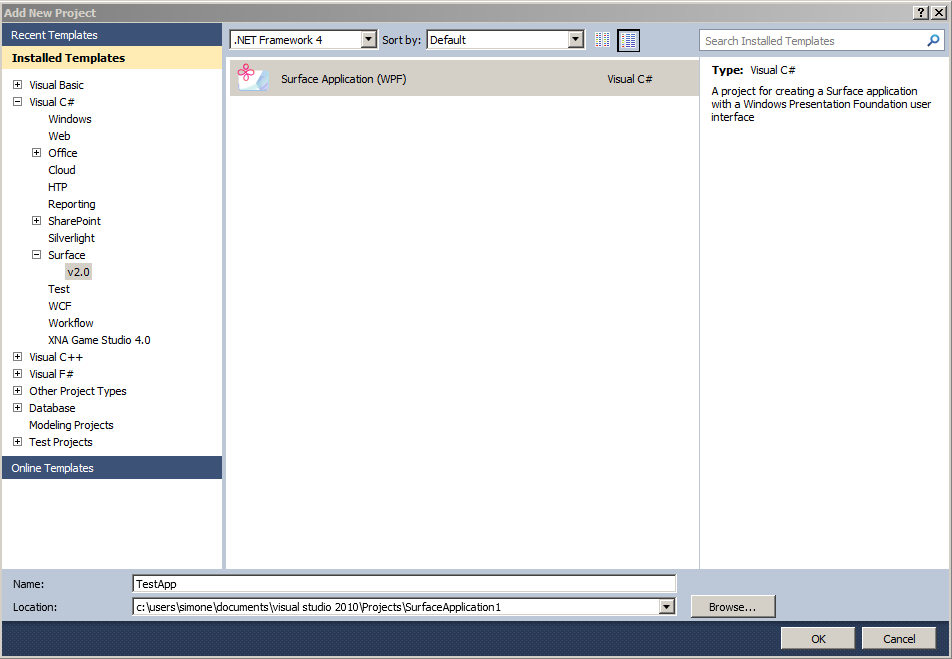
\includegraphics[width=1.0\textwidth]{createProj.png}
  \caption{Create a WPF project}
  \label{fig:createProj}
\end{figure}

\begin{figure}[H]
  \centering
  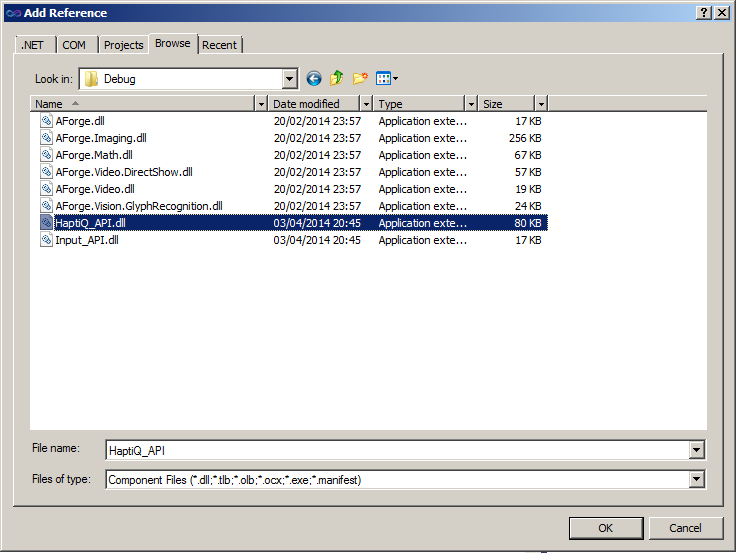
\includegraphics[width=1.0\textwidth]{addreference.png}
  \caption{Add reference to HaptiQ API}
  \label{fig:addref}
\end{figure}

The API contains a multitude of functionality. For more information it is suggested to use Visual Studio, which allows easy access to the documentation for the API. 

\subsection{HapticShapes}

The API supports the following HapticShapes:

\begin{itemize}
\item Rectangle
\lstset{style=sharpc1}
\begin{lstlisting}
HapticShape rectangle = new HapticRectangle(x, y, width, height);
\end{lstlisting}

\item Circle
\lstset{style=sharpc1}
\begin{lstlisting}
HapticShape circle = new HapticCircle(x, y, radius);
\end{lstlisting}

\item Link
\lstset{style=sharpc1}
\begin{lstlisting}
HapticShape link = new HapticLink(src, dst, linkHasDirection);
\end{lstlisting}

\item Line
\lstset{style=sharpc1}
\begin{lstlisting}
HapticShape line = new HapticLine(new Point(x, y), new Point(x_1, y_1));
\end{lstlisting}

\item Polyline
\lstset{style=sharpc1}
\begin{lstlisting}
List<Point> points = new List<Point>();
points.Add(new Point(x, y));
...
HapticShape polyline = new HapticPolyline(points);
\end{lstlisting}

\end{itemize}

HapticShapes are created for WPF applications. However, client applications can implement the \textit{IHapticObject} interface to support tactile objects for XNA application as well.

\subsection{Extending the API}

The API provided does not consider all possible types of applications users may want to implement. However, it is possible to extend it to add new functionality. The user can extend the API from the client side without having to modify the API. 

Note that it might be necessary to add a reference to the \textit{Input\_API.dll} when extending HapticShape.

\newpage
\section{Hardware}

The models for the 4-HaptiQ and the 8-HaptiQ can be found in the folder \textit{HaptiQ 3D Models}. Use MakerWare to import the STL files and print all the interested parts. Note that the printing can take up to several hours, based on the 3D printer used. 

\subsection{Hardware needed}

\begin{itemize}
	\item 3D Printer with 1.8mm ABS Plastic or equivalent
    \item 4 Hitech HS-65MG micro servomotors (8 for the 8-HaptiQ)
    \item 1 Phidget AdvancedServoBoard
    \item 1 Phidget InterfaceKit 8/8/8 or equivalent (must support analog input)
    \item 4 Force-Sensing resistors (8 for the 8-HaptiQ)
    \item Screws of various dimensions 
    \item Super glue
    \item Female and male crimps (with slots)
\end{itemize}

\section{Software Listing}

The software used in this project is listed below:

\begin{center}
    \begin{tabular}{ | l | p{3cm} | p{8cm} |}
    \hline
    Software & Description & Available at \\ \hline
    Phidget libraries & Control servos and pressure sensors & http://www.phidgets.com/ \\ \hline
    GRATF & Locate and recognize Glyphs & http://www.aforgenet.com/projects/gratf/ \\ \hline
    Glyphs Studio & Print Glyphs & http://www.aforgenet.com/projects/gratf/ \\ \hline
    Surface SDK 2.0 & Interface with tabletop & http://www.microsoft.com/en-gb/download/details.aspx?id=26716 \\ \hline
    NCalc & Evaluate mathematical functions in FunctionsApp & http://ncalc.codeplex.com/ \\ \hline
    VS2012 & C\# IDE & \- \\ \hline
    MakerWare & 3D Printer Software & https://www.makerbot.com/makerware/ \\ \hline
    SketchUp & 3D Modelling tool & http://www.sketchup.com/ \\ \hline
    SketchUp STL & STL Exporter plugin & http://extensions.sketchup.com/en/content/sketchup-stl \\ \hline
    \end{tabular}
\end{center}

\end{document}